\documentclass[tikz,border=2pt]{standalone}
\usepackage{amsmath}
\usepackage{pgfplots}
\pgfplotsset{compat=1.18}
\usetikzlibrary{arrows.meta}
\begin{document}
% Lighthouse Company (l = 2, h = 2/3, b = 20, K = 50): for each Q the lowest cost c(Q, r) over r
% (r = 5 for Q = 16..23, r = 4 for Q = 24), from the table of Section 5.8; minimum 13.729 at
% (Q, r) = (20, 5); EOQ value sqrt(2 E[D] K / h) = 18.47.
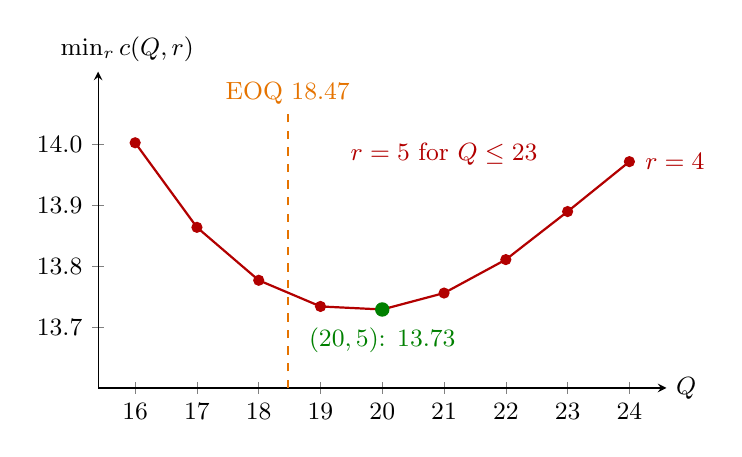
\begin{tikzpicture}[font=\small, >={Latex[length=2mm]}]
  \begin{axis}[axis lines=left, xmin=15.4, xmax=24.6, ymin=13.6, ymax=14.12,
    xtick={16,...,24}, ytick={13.7,13.8,13.9,14.0}, yticklabels={$13.7$,$13.8$,$13.9$,$14.0$},
    xlabel={$Q$}, ylabel={$\min_r c(Q,r)$},
    xlabel style={at={(axis description cs:1,0)}, anchor=west},
    ylabel style={rotate=-90, at={(axis description cs:0,1)}, anchor=south west, xshift=-6mm},
    width=8.8cm, height=5.6cm, clip=false]
    \draw[orange!90!black, thick, dashed] (axis cs:18.47,13.6) -- (axis cs:18.47,14.05);
    \node[orange!90!black, anchor=south] at (axis cs:18.47,14.05) {EOQ $18.47$};
    \addplot[red!70!black, thick, mark=*, mark size=1.6pt]
      coordinates {(16,14.003) (17,13.864) (18,13.777) (19,13.734) (20,13.729) (21,13.756)
                   (22,13.811) (23,13.890) (24,13.972)};
    \addplot[only marks, mark=*, mark size=2.4pt, green!50!black] coordinates {(20,13.729)};
    \node[green!50!black, anchor=north] at (axis cs:20,13.715) {$(20,5)$: $13.73$};
    \node[red!70!black, anchor=west] at (axis cs:24.1,13.972) {$r=4$};
    \node[red!70!black, anchor=south] at (axis cs:21,13.95) {$r=5$ for $Q\leq23$};
  \end{axis}
\end{tikzpicture}
\end{document}
